\chapter{Analysis of Social Navigation in Modern Web Sites}
\label{chapter:analysis}

This chapter includes a survey and analysis of the most interesting
data we've collected which can be found in its whole in
\appendixref{content.inventory}. When we're referencing to \abbr{ID}s we're
using the identifier in the tables found at the specified pages.

\section{Flickr}
\label{section:analysis.flickr}

\sidefigure[Flickr Photo Meta-data]{%
  Photo Meta-data,
  retrieved October 28, 2007, from
  \url{http://flickr.com/photos/benbengraves/187609810/}.
  \label{figure:scrsh.flickr.photo.detail.metadata}
}{%
  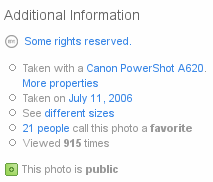
\includegraphics[width=0.9\marginparwidth]{scrsh_flickr_photo_metadata}
}

Flickr is a photo sharing site which are known to be on the cutting edge when
it comes to enabling new and innovating features in its domain. Flickr has a
quite peculiar history as it started out as a massively multi player online
game. An environment for photo sharing within the game was added in 2004 which
quickly became more popular than the game itself. The focus of the company was
shifted and their new photo sharing community was bought by Yahoo! Inc. in
March 2005 \citep[\p{257}]{livingston07}.

This subsequent
analysis of Flickr will be carried out as a registered user. One has to be
registered for interacting with the site in such a way that one leaves
persistent traces. The site has a open nature enabling anonymous access
to the majority of content.

\subsection{Thumbnails}

Already on the welcome page (\figureref{scrsh.flickr.welcome})
we're finding navigation links that are social of
nature. Four thumbnails functions as sample of the most recently uploaded
photos by other members of the community. One can either navigate straight to
a detailed page for each particular photo by clicking on the respective
thumbnail \flickrref{6}
or the profile of the uploader by clicking on their user
name \flickrref{7}. Such thumbnails
with minimal meta data (the uploader) are prevalent all over Flickr. Of the
120 pages we collected in our content inventory 26 of them contained
thumbnails. Most of these thumbnails
are giving users incentives to navigate using social means%
\sidenote{%
  Apart from the few pages that only show a
  stream of your own thumbnails when you're browsing your
  own photos by various methods.
}.
Which photos these thumbnails portray is dynamic. That is to say that other
users' actions\dash{}uploading a photo, tagging a photo, taking a photo with a
specific camera, collecting photos into sets, and adding photos to a certain
group\dash{}all determine the navigational choices you as a user is
presented with.

\subsection{Meta-data}

We arrive on a photo detail page as in
\figureref{scrsh.flickr.photo.detail}
if we utilize one of these thumbnails for navigation. In addition to comments
on the photo we find meta-data as in 
\figureref{scrsh.flickr.photo.detail.metadata}
Meta-data include the date the photo was taken, the manufacturer and the model
of the camera that was used which are all so called Exif%
\sidenote{%
  Exchangeable Image File: a specification for image file format used
  in digital cameras.
}
data. Flickr utilize this data by enabling navigation based both on the
dates a picture was taken and by camera make and model. Say you're trying to
find a picture from your home town on a particularly beautiful summer day. By
using date of picture taking based navigation coupled with tags or
geographical data (which both will be discussed shortly) you're probably
increasing you chances of finding what you want. Camera make information could
be useful when looking at the quality of pictures taken with certain cameras
before purchasing one yourself.

\begin{figure}
  \captionstyle{\raggedright}
  \begin{whole}
    \begin{minipage}[t]{0.475\wholewidth}
      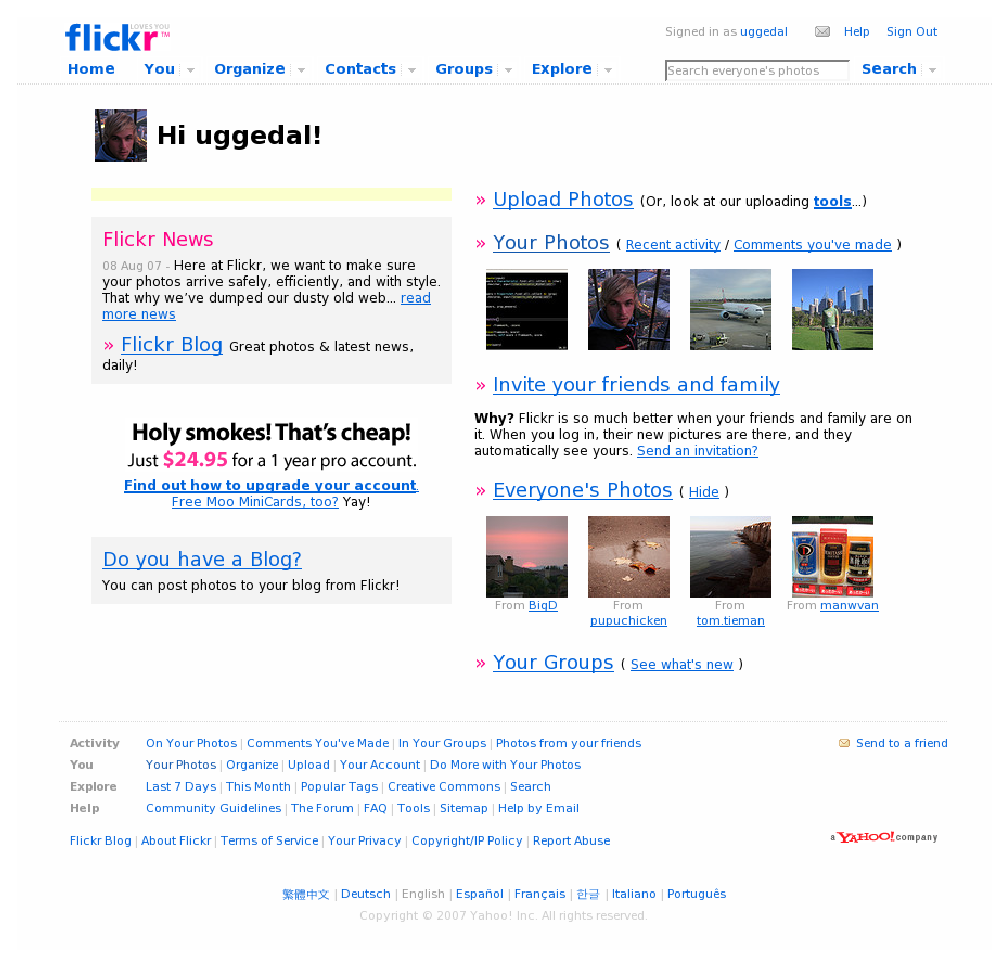
\includegraphics[width=\textwidth]{scrsh_flickr_welcome}
      \caption[Flickr Welcome Page]{%
         The Welcome Page of Flickr,
         retrieved October 16, 2007, from \url{http://flickr.com}.}
      \label{figure:scrsh.flickr.welcome}
    \end{minipage}
    \hfill
    \begin{minipage}[t]{0.475\wholewidth}
      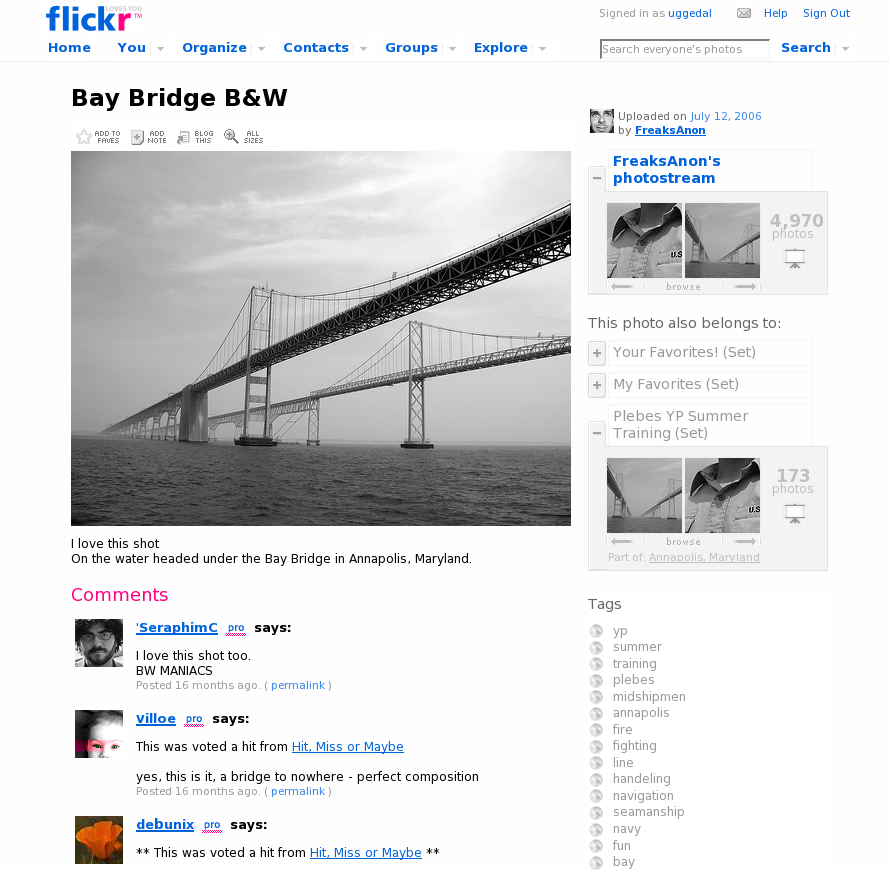
\includegraphics[width=\textwidth]{scrsh_flickr_photo_detail}
      \caption[Flickr Photo Detail Page]{%
         A Photo Detail Page on Flickr,
         retrieved October 26, 2007, from
         \url{http://flickr.com/photos/benbengraves/187609810}.}
      \label{figure:scrsh.flickr.photo.detail}
    \end{minipage}
  \end{whole}
  \normalcaption
\end{figure}

\subsection{Folksonomy}
Of most importance
for Flickr, and indeed what makes Flickr a folksonomy, is its tagging
abilities. Caterina Fake, co-founder of Flickr, explains its importance as
\postquote[\p{261}]{livingston07}{%
  Tagging really revolutionized the way the product behaved}
All registered user can label anyone's photos by applying such short
descriptive tags. This collaborative process lay the ground work for other
user's ability to easily browse photos by topic.
\figureref{scrsh.flickr.tagcloud}
exemplifies how the user generated data trough tagging can be used as a
navigational aid. A so called \term{tag cloud} is used to visualize the
popularity (and thereby importance) of the individual tags. The larger the
tag title, the more frequent the tag has been applied to photographs.

\begin{figure}
  \begin{whole}
    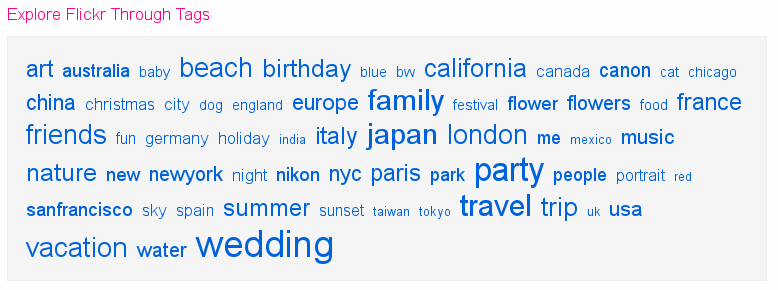
\includegraphics[width=\wholewidth]{scrsh_flickr_tagcloud}
    \caption[Flickr Tag Cloud]{%
       Tag Cloud,
       retrieved November 1, 2007, from \url{http://flickr.com/explore}.}
    \label{figure:scrsh.flickr.tagcloud}
  \end{whole}
\end{figure}

Tag clustering was released in the fall of 2005 \citep{butterfield05} as a way
to easier see the relationships between separate tags. For any given tag a
cluster of three related tags is generated and displayed to users when they
are browsing as seen in
\figureref{scrsh.flickr.photo.detail}.
Flickr algorithmically generates these listings based on what tags users tend
to use together for labeling a photo.

\begin{figure}
  \begin{whole}
    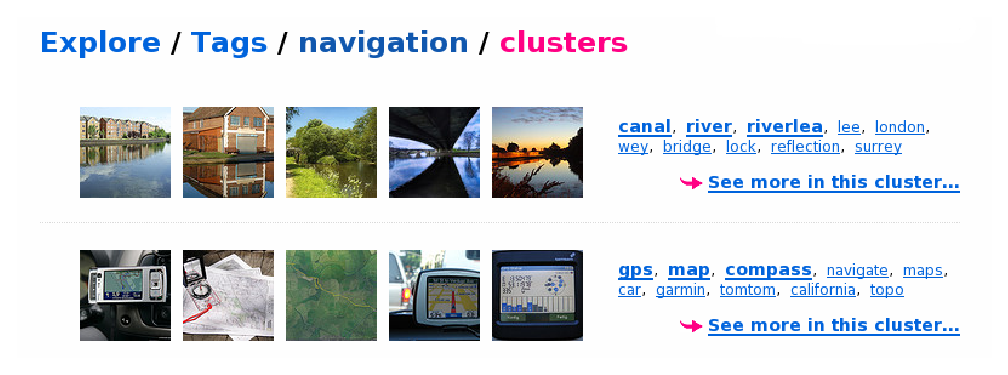
\includegraphics[width=\wholewidth]{scrsh_flickr_tagcluster}
    \caption[Flickr Tag Cluster]{%
       Tag Cluster,
       retrieved November 19, 2007, from
       \url{http://flickr.com/photos/tags/navigation/clusters/}.}
    \label{figure:scrsh.flickr.tagcluster}
  \end{whole}
\end{figure}

Tagging is a very flexible approach only hindered by users' imagination. In
the early days of Flickr there was no support for geographical data. Users
soon found a remedy for this by tagging photos with longitude and latitude.
By using the same technology we're using in our prototype application
(Greasemonkey) they were able to integrate Google Maps%
\sidenote{
  Available at \url{http://maps.google.com}
} in Flickr, enabling user's to place their photos on a map and automatically
generate geographical coordinate tags%
\sidenote[2]{
  More info about the early days of \term{geotagging} can be found on the
  remains of the Flickr Geotagging group, available at
  \url{flickr.com/groups/geotagging/}.
}.

\subsection{Geographical Data}

In late August 2006 Flickr introduced geotagging abilities
\citep{butterfield06a} by integrating mapping aspects from Yahoo! Maps%
\sidenote{
  Available at \url{http://maps.yahoo.com}.
}
Users could now place their photos on a
map to signify where they were captured without resorting to clever hacks of
the standard tagging system.

\figureref{scrsh.flickr.geotagged} shows how one of the authors photos are
placed on a map \flickrref{1.1.6}.
One can then cycle trough the adjecent photos of other users
that are interesting (see
\sectionref{analysis.flickr.interestingness}) or recently published.
What we see here is indirect social navigation where the advice is explicitly
given. When a user places his photo geographically on a map he makes available
navigational choices for other users who for some reason are interested in
that particular geographical area. Such visualizations of geographic
navigation clues are a good example of social texture.

\begin{figure}
  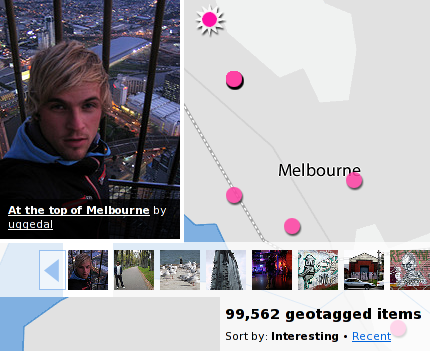
\includegraphics[width=0.8\textwidth]{scrsh_flickr_geotagged}
  \caption[Flickr Geotagging]{%
     Geotagging on Flickr,
     retrieved March 3, 2008, from
     \url{http://flickr.com/photos/uggedal/261824261/map/?view=everyones}.}
  \label{figure:scrsh.flickr.geotagged}
\end{figure}

\subsection{Interestingness}
\label{section:analysis.flickr.interestingness}

The concept of \term{interestingness} was introduced by Flickr during
the same time tag clustering was unveiled \citep{butterfield05}.

Interestingness is a rating of how interesting a photograph is based on
how many views the photograph has, how many users have favorized the
photograph, and how many comments a photograph have. Fovirization have the
highest weight, comments medium weight, and views the least weight
in the algoritm that generates the interestingness rating \citep{dean08}.
Users are not aware of the score of a particular photograph's interestingness,
but the highest rated photographs are available trough the \q{Explore} part of
Flickr
(\flickropenref{5.3}
\flickropenref{5.4}).

The interestingness system is a great example of passive and indirect social
navigation. Based on the behaviour of other users the more interesting photos
are made more visible in Flickr's interface. Flickr can be seen as a
collaborative filtering system in which uses implicit ratings. When a user
leaves a comment on a photo the aim is likely to voice his reactions to the
picture, and not vote the picture down or up. Interestingly Flickr uses
collaborative filtering without personalization of it's recommendations and
rather gives the whole pupulation the same recommendations.
The use of interestingness seem
to have worked well for Flickr as users are trying hard to make their photos
receive higher interestingness scores.
As of this writing a pattent on interestingness is pending
\citep{butterfield06b}.

\section{Facebook}
\label{section:analysis.facebook}

Facebook is a social network site that started as a service only available for
Harvard students in February of 2004. Within the same month Facebook was
opened up for students at several other universities in the
US. More universities and colleges were supported and Facebook opened up it
doors for high-school students in September of 2005 \citep{cassidy06}
before allowing global access for anyone\dash{}student or not\dash{}in
September of 2006 \citep{abram06}.
Facebook has seen an enormous growth and are today the largest social network
in some countries (see
\sectionref{background.sociality.the.social.web.social.network.sites}).

\subsection{Profiles}

As we've seen pictures and their thumbnails and titles are central in Flickr.
In the same way user names and thumbnails of profile images are scattered all
trough Facebook. This is no mystery as the dominant entity of Facebook is
people and their profiles much as pictures' essentialness for Flickr.

\begin{figure}
  \begin{whole}
    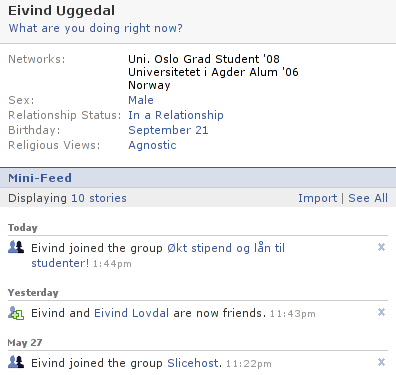
\includegraphics[width=\wholewidth]{scrsh_facebook_profile}
    \caption[Facebook Profile]{%
       Author's profile page on Facebook,
       retrieved May 30, 2008, from
       \url{http://www.facebook.com/profile.php?id=903795175}.}
    \label{figure:scrsh.facebook.profile}
  \end{whole}
\end{figure}

\subsection{News Feed}
\label{section:analysis.facebook.news.feed}

The landing page when you log in to Facebook after having configured your
account is the \q{News Feed} \facebookref{0}.
The news feed shows the recent activities your
friends have conducted. This eliminates the tedious process of checking every
profile page of your friends to keep on top of what they're up to.
The feed shows a list of items, each representing a type of activity. As
shown in \figureref{scrsh.facebook.news.feed}
these activities are distinguished by an
icon and presented chronologically. The data presented in the news feed are an
aggregation of every friend's \q{Mini-Feed} located on their profile page
\facebookref{1} as seen in \figureref{scrsh.facebook.profile}.

The news feed enables social navigation. All the navigational choices the feed
of representations of activity presents are constructed as a by-product of
other people's actions. When you select to attend an event, join a group,
post a photo, change your relationship settings, befriend a person, post a
comment on a wall or photo, or update your profile information your action
is added to the feed. The navigation presented by the feed
is therefore indirect and passive social navigation provided by implicit
feedback\dash{}providing no additional overhead for the advice provider.

\begin{figure}
  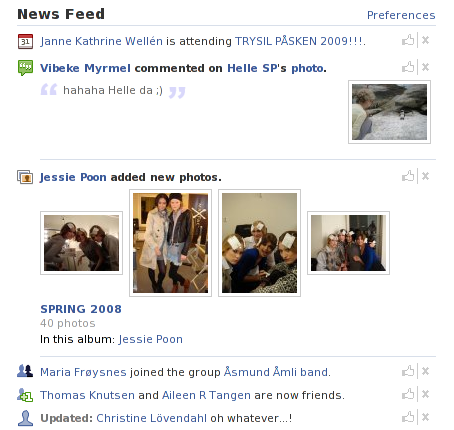
\includegraphics[height=0.9\textheight]{scrsh_facebook_news_feed}
  \caption[Facebook News Feed]{%
     Author's news feed on Facebook,
     retrieved March 26, 2008, from \url{http://www.facebook.com/home.php}.}
  \label{figure:scrsh.facebook.news.feed}
\end{figure}


\subsection{Hyperlink Sharing}

Facebook have an interesting feature that makes hyperlink sharing easier for
it's users. When one are posting a comment on a the wall of a person
\facebookref{1.19.1},
group
\facebookref{1.1.3.1.1.9},
or event
\facebookref{1.1.3.2.1.9}
one can provide a \abbr{URL}. By providing such a hyperlink to a
third party web page Facebook extracts an excerpt of the linked page with
optional graphics as seen in \figureref{scrsh.facebook.wall.link}. Since the
recipient of a message with a hyperlink can respond to the advice provider
we're witnessing active and direct social navigation with
improved \abbr{URL} handeling as envisioned by
\citet[\p{811}]{dieberger97}.

\begin{figure}
  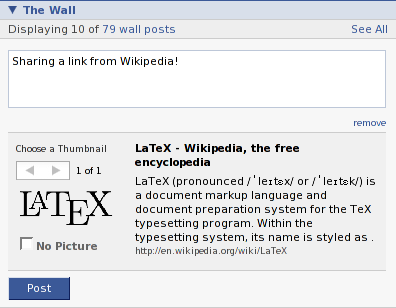
\includegraphics[width=0.8\textwidth]{scrsh_facebook_wall_link}
  \caption[Facebook Hyperlink Sharing]{%
     Sharing of hyperlinks on Facebook,
     retrieved June 2, 2008, from
     \url{http://www.facebook.com/profile.php?id=903795175}.}
  \label{figure:scrsh.facebook.wall.link}
\end{figure}

\subsection{Photo Tagging}

Photos on Facebook can be tagged \facebookref{1.19.1} like those on Flickr.
But as you can see in \figureref{scrsh.facebook.photo.tagging} one are
tagging with persons as identifiers on Facebook instead of keywords as on
Flickr. We are
therefore not witnessing a folksonomy on Facebook. Photo tagging on Facebook
can be used as a means of navigating photos of particular individuals or
navigating towards people based on photos with various taggings of
individuals.

\begin{figure}
  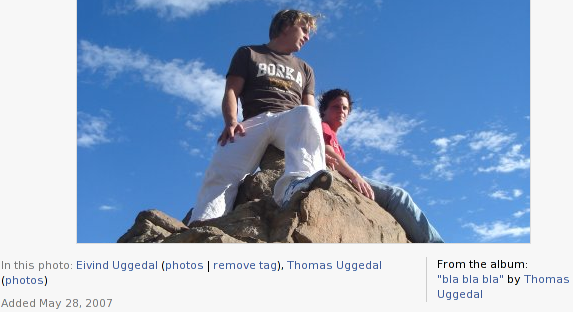
\includegraphics[width=0.9\textwidth]{scrsh_facebook_photo_tagging}
  \caption[Facebook Photo Tagging]{%
     Photo tagging on Facebook,
     retrieved June 2, 2008, from
     \url{http://www.facebook.com/photo.php?pid=177290&id=579356186}.}
  \label{figure:scrsh.facebook.photo.tagging}
\end{figure}
